\documentclass{article}

\usepackage{../parm}
\begin{document}

    \section{Pour aller plus loin}

    \subsection{Compilation de code C}
    Avec le jeu d'instructions de ce processeur, il est possible d'exécuter du code C compilé par \texttt{Clang}.
    Il doit cependant rester relativement simple avec une structure bien précise.

    En particulier, on évitera:
    \begin{itemize}
        \item Les appels de fonctions (\texttt{LR}, \texttt{PUSH}, \texttt{POP} non implémentés)
        \item Les variables globales et \texttt{static} (adressage uniquement sur la pile)
        \item Les adressages indirects (donc l'utilisation de tableaux ou de chaînes)
    \end{itemize}

    On s'assurera donc:
    \begin{itemize}
        \item D'écrire tout le code dans la fonction \texttt{void run()}
        \item De déclarer toutes les variables dans le corps de cette dernière
    \end{itemize}
    
    Voici le code de démarrage pour un programme C dans le cadre du projet :
    \lstset{
        basicstyle=\ttfamily,
        keywordstyle=\color[rgb]{0,0,1},
        commentstyle=\color[rgb]{0.133,0.545,0.133},
        stringstyle=\color[rgb]{0.627,0.126,0.941},
        frame=single,
        tabsize=4,
        columns=fixed,
        breaklines=true,
        xleftmargin=0pt,
        postbreak=\mbox{\textcolor{red}{$\hookrightarrow$}\space},
    }
     \begin{lstlisting}[language=C]
#include <parm.h>

void run()
{
	BEGIN();
	// code ici	
	END();
}
    \end{lstlisting}
    
    On utilise ici une fonction s'appelant \texttt{run} et non pas \texttt{main} car les compilateurs C émettent un warning lorsque la fonction \texttt{main()} ne se termine pas (par exemple, si elle contient une boucle infinie). Or, c'est ici un cas souhaité, et appeler la fonction autrement évite ce warning.
    
    Les appels \texttt{BEGIN} et \texttt{END} sont des macros servant à allouer l'espace mémoire nécessaire pour gérer les périphériques d'entrée/sortie. Il faut systématiquement les écrire dans vos programmes en début et en fin de fonction, sans quoi vous ne pourrez pas utiliser la RAM et ne pourrez donc pas utiliser de variables.

    La commande à utiliser est la suivante (écrivez la, si vous la copiez depuis le PDF les caractères ne seront pas bons) :
    \begin{lstlisting}
clang -S -target arm-none-eabi -mcpu=cortex-m0 -O0 -mthumb -nostdlib -I./include main.c
    \end{lstlisting}
    avec \texttt{main.c} le fichier source C. Veillez à être dans le dossier code\_c en lançant cette commande.

    Cela crééra un fichier de sortie \texttt{main.s} contenant les instructions assembleur, entourées de directives spéciales qui ne nous intéressent pas ici.

    \paragraph{Remarque 2:} depuis la version 9 de \texttt{Clang}, l'addressage mémoire est réalisé différemment en utilisant des instructions \texttt{add <Rd>,SP,\#<imm8>} et \texttt{ldr <Rt>,<Rn>,\#<imm5>} qui ne sont pas prises en charge par l'implémentation.
    Il faut donc s'assurer d'utiliser une version 4 à 8 de \texttt{Clang} (paquet \texttt{clang-8} sous Ubuntu).

    Le code assembleur devra être passé à l'assembleur écrit dans le cadre du projet pour générer le fichier lisible par Logisim et pouvoir l'importer dans la ROM.
    
    \subsection{Périphériques d'entrée/sortie mappés en mémoire}
    
    Actuellement, notre processeur ne peut interagir avec l'utilisateur que de façon très primitive :
    \begin{itemize}
	    \item En écrivant une valeur dans un registre
	    \item En lisant ou écrivant une valeur dans la RAM
    \end{itemize}
    
    Dans les deux cas, cela limite à des valeurs numériques, et cela implique de prévoir à l'avance, par convention, dans quel registre ou case mémoire lire ou écrire.
    
    Dans la réalité, vous lisez ce document sur un ordinateur avec lequel vous interagissez via des périphériques d'entrée/sortie : un clavier, une souris, un écran, etc.
    
    Deux méthodes sont principalement utilisées pour gérer de tels périphériques :
    
    \bgroup
    \def\arraystretch{1.5}%  1 is the default, change whatever you need
    \begin{tabularx}{\textwidth}{|X|X|}
    	\hline
    	Entrées/sorties mappées en mémoire (MMIO) & Entrées/sorties mappées en ports (PMIO) \\
    	\hline
    	L'espace mémoire de l'ordinateur contient des sections correspondant non pas à une vraie mémoire, mais à des registres partagés avec des périphériques & Chaque périphérique possède un ou plusieurs "ports" qui lui sont associés, chacun ayant un numéro correspondant, et le processeur possède des instructions spécifiques permettant de lire ou d'écrire dans ces ports \\
    	\hline
    	Utilise les instructions de gestion de RAM & Utilise des instructions spécifiques (ex: \texttt{in} et \texttt{out} en x86 \\
    	\hline
    	Game Boy, [S]NES, Commodore 64, anciens périphériques PC & Compatibles PC modernes (PCs, Macs, smartphones, ...) \\
    	\hline
    \end{tabularx}
    \egroup
    
    De nos jours, c'est l'approche MMIO qui est généralement préférée. L'approche PMIO était très pertinente à l'époque où la mémoire physique était limitée, et où "perdre" une partie de l'espace mémoire en échange de périphériques était trop coûteux. De nos jours, les bus d'adresse de moins de 16 bits se font rares excepté sur les microcontrôleurs, et le PMIO n'est plus utilisé que dans certains cas pour des raisons de compatibilité (ex: port série ou parallèle sur PC).
    
    Le processeur PARM possède une RAM de 256 mots de 32 bits et un bus d'adresse sur 9 bits. Son espace mémoire est disposé de la manière suivante :
    
    \newcommand{\memsection}[4]{
		\bytefieldsetup{bitheight=#3\baselineskip}	% define the height of the memsection
		\bitbox[]{8}{
			\texttt{0x\uppercase{#1}}	 % print end address
			\\ \vspace{#3\baselineskip} \vspace{-2\baselineskip} \vspace{-#3pt} % do some spacing
			\texttt{0x\uppercase{#2}} % print start address
		}
		\bitbox{16}{#4} % print box with caption
	}
	
	\begin{bytefield}{24}
	\begin{rightwordgroup}{mémoire virtuelle}
		\memsection{1ff}{110}{3}{-- inutilisé --}\\
		\memsection{10f}{100}{4}{Ports I/O}
	\end{rightwordgroup}\\
	\begin{rightwordgroup}{mémoire physique}
		\memsection{0ff}{000}{4}{Pile}
	\end{rightwordgroup}\\
\end{bytefield}

	Les 256 premiers mots (adresses $[0;256[$) correspondent à la mémoire RAM physique, tandis que les 256 suivants sont "virtuels", ils sont gérés par le contrôleur MMIO présent en bas du circuit, qui se charge de déléguer aux différents périphériques. Ici, 16 emplacements sont alloués, donc les adresses $[256;271[$ correspondent à des périphériques et les adresses $[271;512[$ ne sont "branchées" à rien.
	
	La documentation des différents périphériques est disponible dans le fichier \texttt{include/parm.h}.
	
	\subsubsection{Exemple : DIP switch}
	
	Un composant d'entrée très courant est le DIP switch. Il s'agit d'un petit bloc comportant une série de $n$ interrupteurs, encodant un nombre sur $n$ bits. Voici à quoi ça ressemble :
	
	\begin{figure}[t]
        \begin{center}
            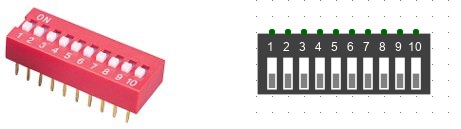
\includegraphics[width=250pt]{pictures/dip.png}
            \caption{\label{fig_dip_switch}DIP switch}
        \end{center}
    \end{figure}
    
    Notre processeur est relié à trois switches de ce genre, sur les entrées 3, 4 et 5 (adresses 259, 260 et 261). Du point de vue d'un programme, lire depuis les DIP switches revient à lire depuis une variable qui serait stockée à ces emplacements, c'est entièrement transparent.
    
    \subsubsection{Exemple : Terminal}
    
    La manière la plus simple d'afficher du texte est via un terminal. Nommé d'après les terminaux physiques qui équipaient les mini-ordinateurs des années 1970, son fonctionnement est simple : quand il reçoit un caractère, il l'affiche. Certains caractères ont un effet particulier :
    \begin{itemize}
    	\item \texttt{\textbackslash n} (newline) effectue un retour à la ligne
    	\item \texttt{\textbackslash b} (backspace) efface le dernier caractère saisi
    	\item \texttt{\textbackslash f} (form-feed) efface l'écran
    \end{itemize}
    Ainsi, ça évite d'avoir des entrées spécifiques pour toutes ces actions.
    
    En pratique, le terminal de Logisim possède plusieurs entrées : l'horloge, le caractère, la mise à jour et la réinitialisation. Cette dernière n'est utilisée que quand on appuie sur le bouton "Reset" du processeur.
    
    À chaque front montant d'horloge, si la broche "mise à jour" est haute, alors le caractère est affiché.
    
    Une seule sortie est fournie aux programmes : caractère. Sa valeur est reliée à l'entrée "caractère" de l'écran, et dès qu'une écriture est faite dans cette sortie, l'entrée "mise à jour" est passée à 1.
    

\end{document}